\documentclass{article}

\usepackage[T1]{fontenc}
\usepackage[utf8]{inputenc}
\usepackage{mdwlist} % To have compact lists
\usepackage{hyperref} % To have links to URLs
\usepackage{float} % To force images to the right place
\usepackage{listings} % To display source code

\usepackage{caption}
\usepackage{subcaption}

% To include images
\usepackage{graphicx} 
\graphicspath{ {images/} } % location of images

% Disables automatic indents globally
%\setlength{\parindent}{0pt}


\begin{document}

% - - - - Header Begins - - - -
\begin{center}
	{\LARGE \textbf{Project Plan}} \\
	\vspace{0.5em}
	\textsl{Team $\lambda$ Lovelace}
\end{center}

\vspace{0.5em}

\begin{center}
	10th June 2016 \\
	COMP47250, Team Software Project 2016 \\ 
	University College Dublin, Ireland \\
\end{center}

\vspace{0.5em}
% - - - - Header Ends - - - -

% Executive summary
%\renewcommand{\abstractname}{Executive Summary}
%\begin{abstract}
%\noindent A collaborative recommender system for tweets; a more personalised tweet stream.
%\end{abstract}


\noindent This is a project plan for the team $\lambda$ Lovelace\footnote{pronounced: Lambda Lovelace}, summer 2016. The module formally started 2016.05.16 and will end in a final code \& report submission 2016.08.19. Four weeks have passed when this document was submitted.

It is assumed the reader is familiar with Twitter. If not there is a short appendix at the end of this document detailing few of the main features.


\section{Vision}

Our project is about creating a collaborative recommender system for tweets or in other words: a personalised stream of tweets. Tweets that are more relevant or interesting would be shown first while unrelevant ones would be deferred to later. Tweets from non-followers may be suggested as well.
\\\\
On a high level there are two main components to the project:

\begin{itemize*}
	\item \textbf{Front-end}: iOS Twitter mobile app
	\item \textbf{Back-end}: Collaborative recommender system
\end{itemize*}

\noindent It should be noted that after the project started and we did a more thorough review we found out that Twitter already does provide their own feed personalisation. Therefore the project goal was pivoted to provide better recommendations than Twitter already provides.

\begin{figure}[H]
    \centering
    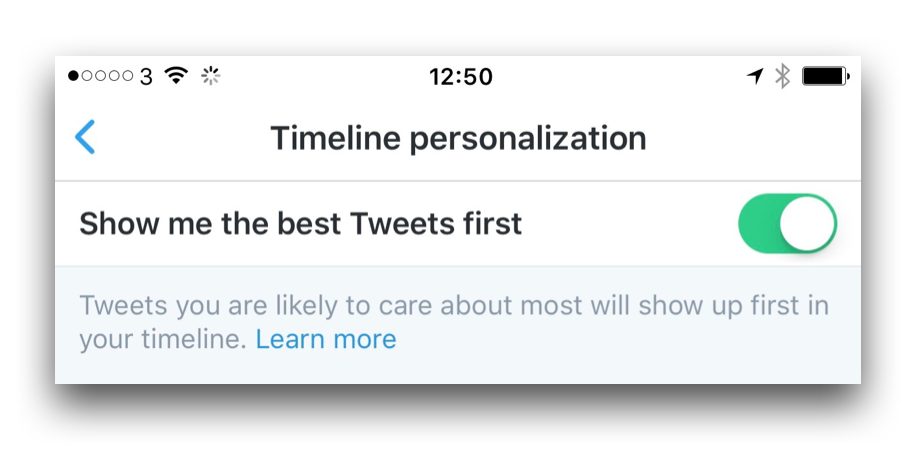
\includegraphics[width=0.6\textwidth]{tp}  
    \caption{Screenshot from the official iOS Twitter app}
\end{figure}


\subsection{Why?}
The premise for our project is the assumption (or observation) that people are experiencing an information overload on Twitter. When a user follows another user on Twitter they subscribe to all their tweets and re-tweets\footnote{Twitter offers the option to turn off re-tweets for a particular followee}. A user may hold interest in programming but dislikes political discussions (or \textit{vice versa}).

\begin{figure}[H]
    \centering
    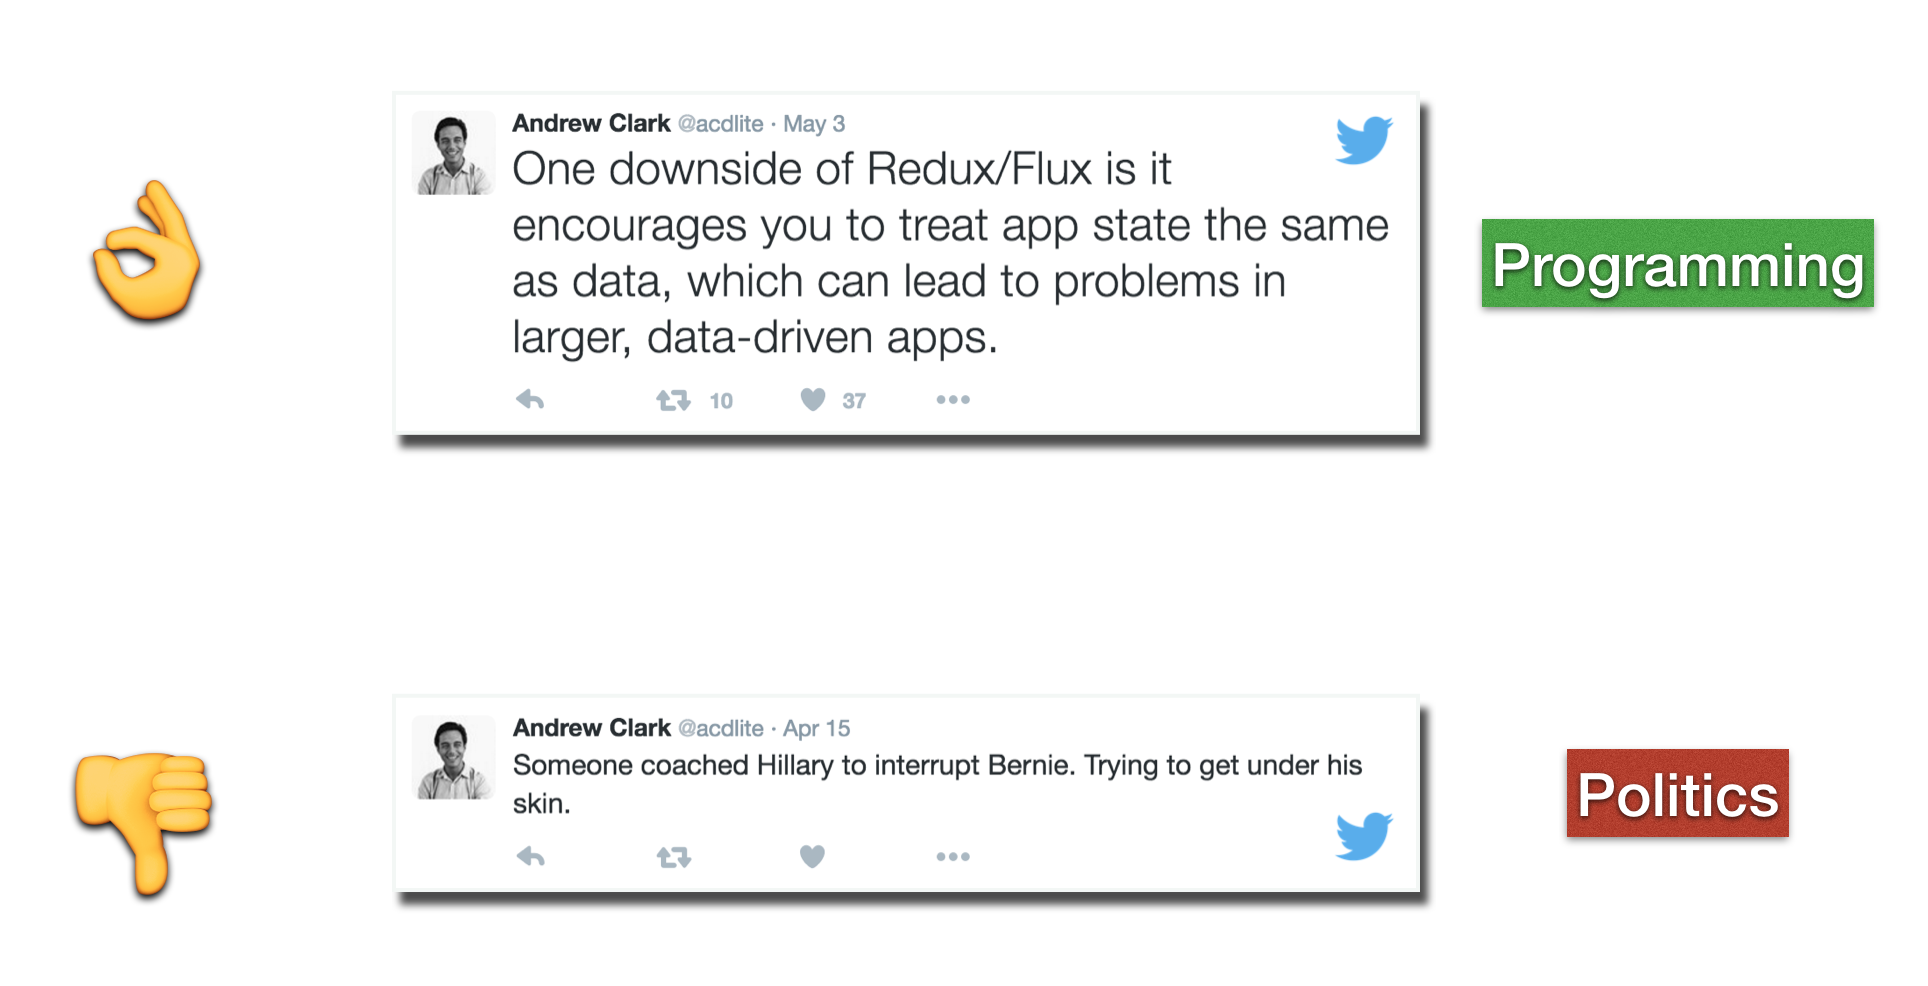
\includegraphics[width=0.8\textwidth]{the_problem}  
    \caption{A Twitter user that tweets about programming and politics}
\end{figure}

The theme for the summer 2016 practicum is \textit{Future Of News}. We believe that the future of news is going to be filtering and delivering personalised content to people. We see personalised tweet streams to be a stepping stone in that direction.

\subsection{Who?}
Our target users are Twitter power users. Such a user follows roughly more than 100 Twitter accounts and has been using Twitter for few weeks or months. More importantly, the user is seeing on a regular basis tweets in his or her feed that are of low relevance.

\subsection{How?}
A Twitter user uses our iOS mobile client and grants us API access. Uninteresting tweets are filtered out (or deferred to later) while interesting tweets are prioritised. Tweets from non-followers may be suggested as well. Our iOS app will make observations of the users engagements (opening, liking, time in focus, etc) and sends the information to the recommender back-end for further recommendations.
\\\\
The mobile app is required in order to collect additional user preference information to refine the recommendations. For example, if a user clicks a link in a tweet, likes a tweet, retweets, or engages in conversations. Another potential passive observation mechanism would be to have the client measure the amount of time a tweet is visible. Thinking being if a tweet is in focus for longer it might be of more interest than a tweet that is scrolled past quickly.



\section{Minimum Viable Product}

\begin{figure}[H]
    \centering
    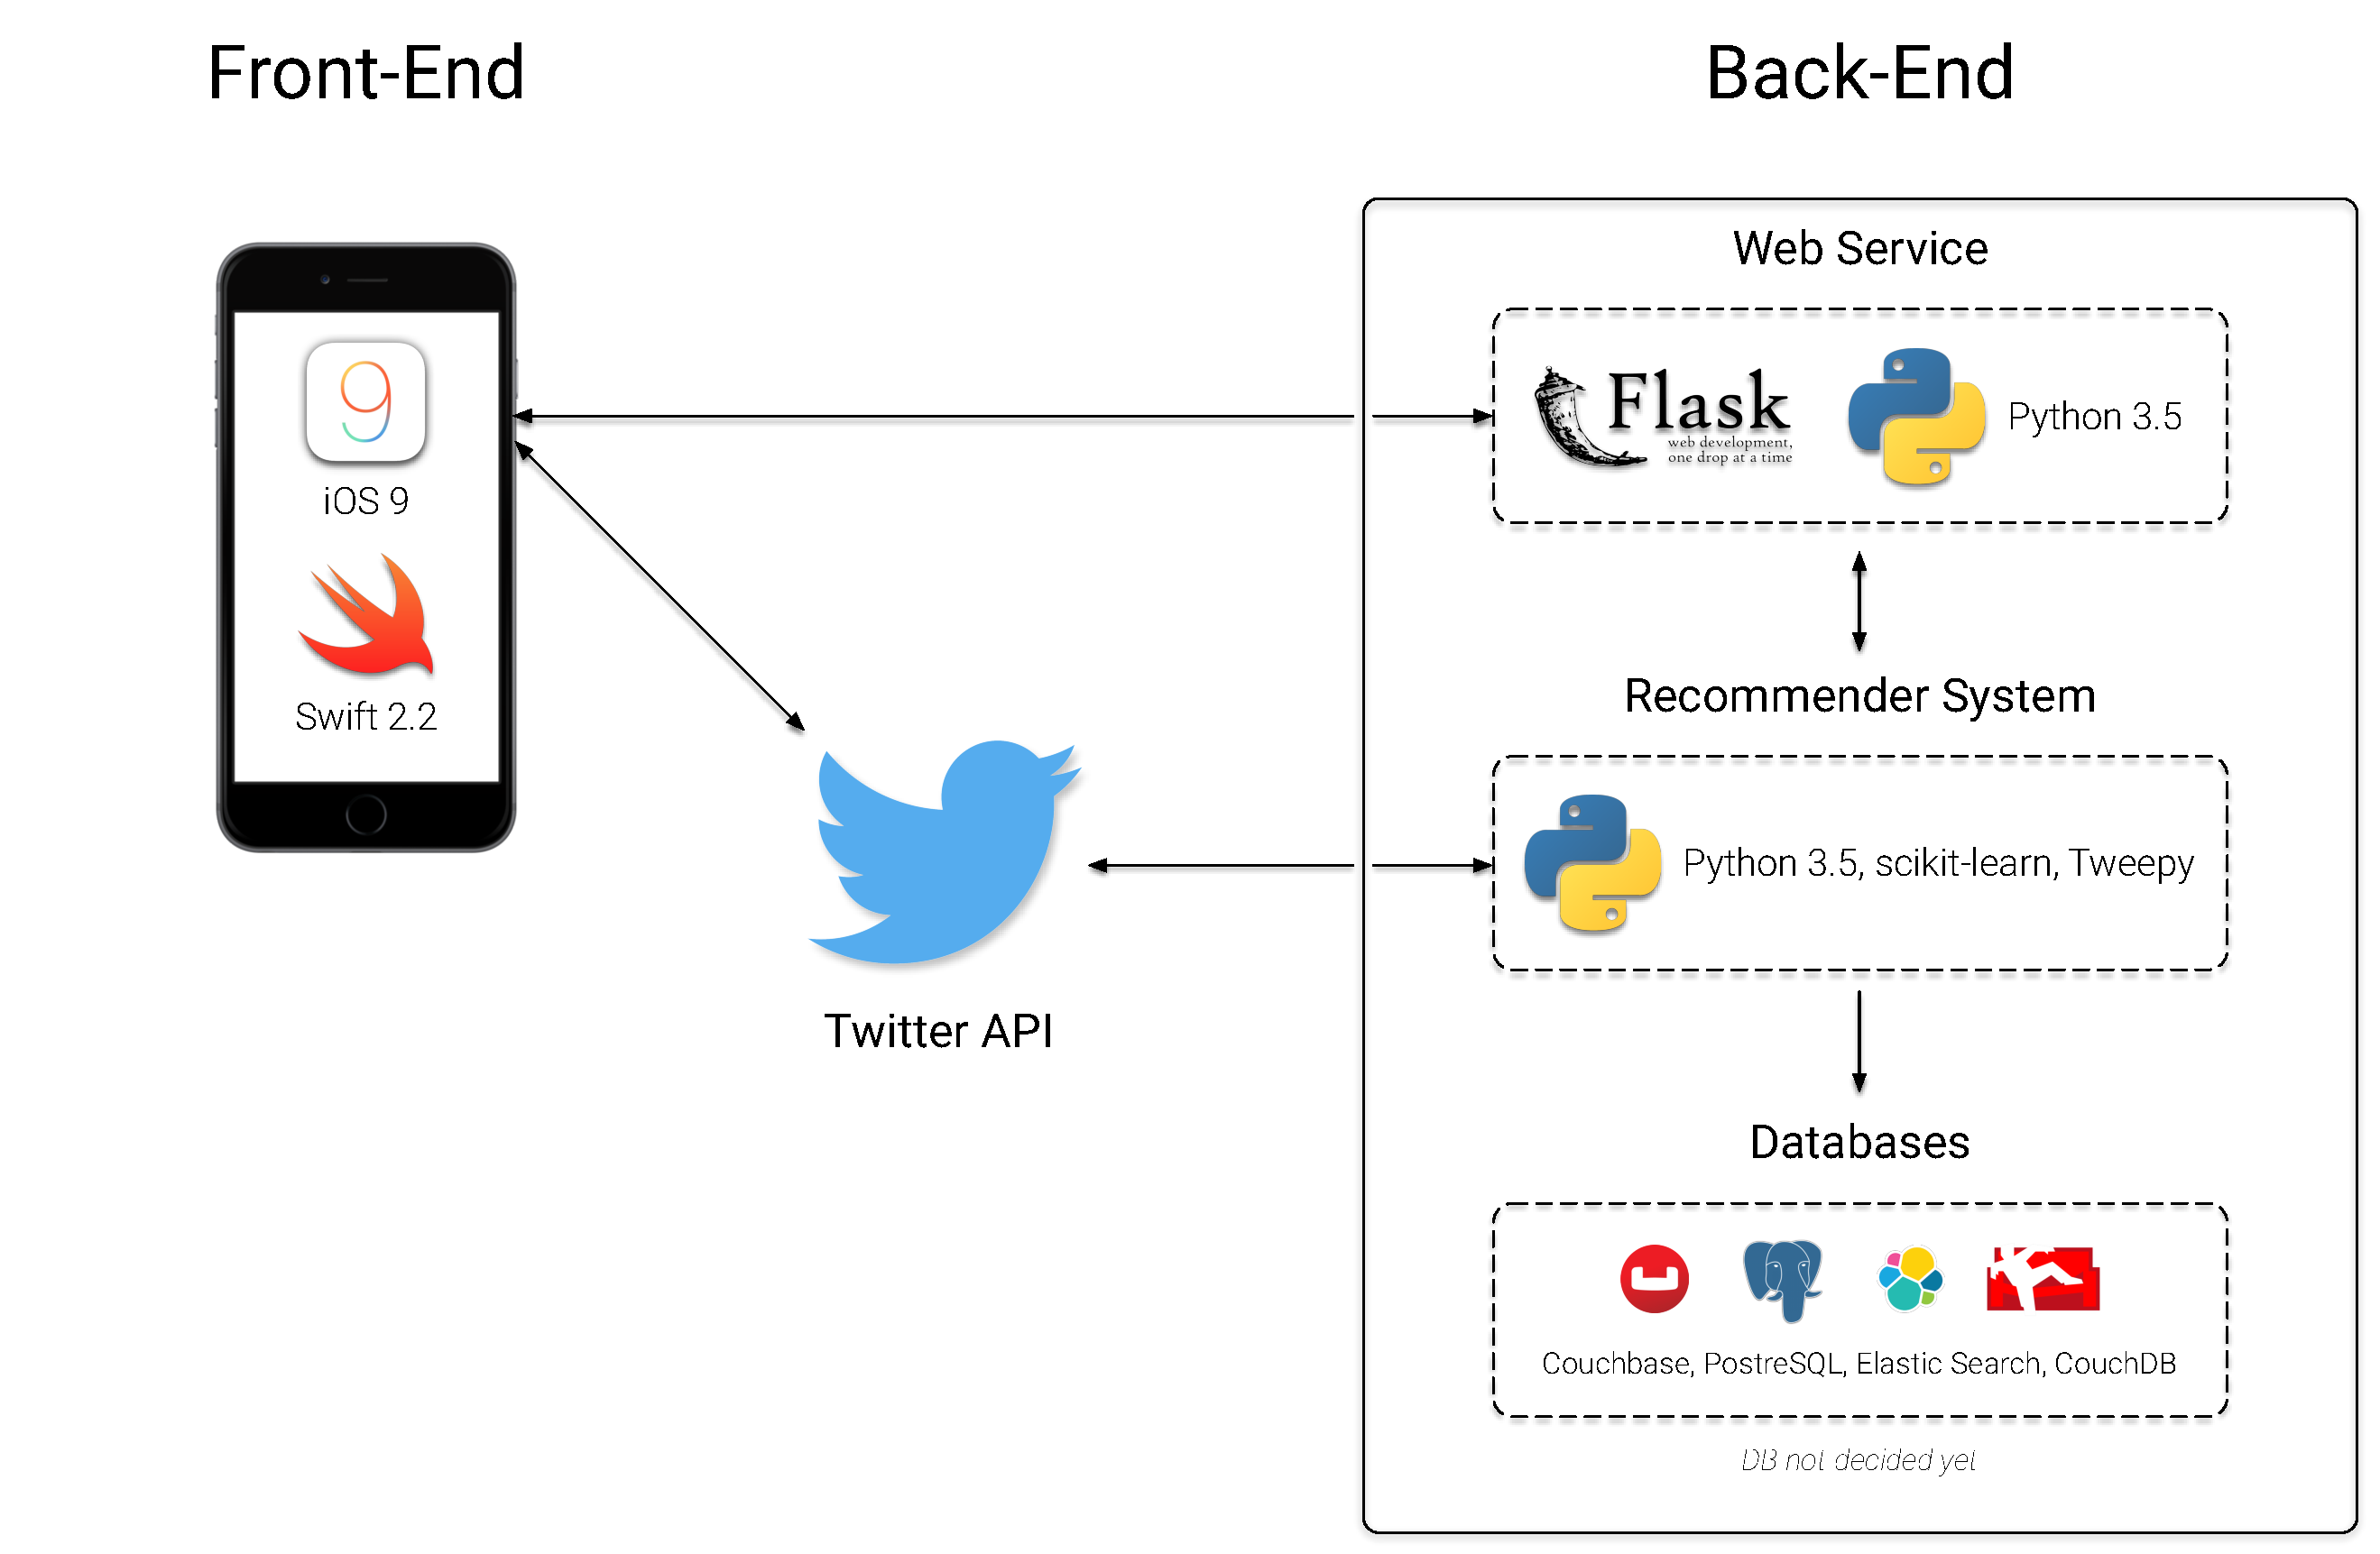
\includegraphics[width=\textwidth]{system_overview}  
    \caption{System overview}
\end{figure}

\subsection{Front-End: iOS}
Our Twitter client acts as a medium to showcase:

\begin{itemize*}
	\item The personalised tweets to the users.
	\item Provide information to the Recommender System some useful data about user interactions with the App, that could potentially help in analysing the user's likes.
\end{itemize*}

\noindent For the MVP we have decided to concentrate in showing the personalised tweets.
The App provides the ‘Sign in’ functionality to have the users permission to access their 
Twitter data. We have used the Fabric - Twitter’s Mobile Development Platform to perform the OAuth Authentication process. After the user has logged in, they can see the personalised tweets with colour code indicating the relevance of tweets to the user's interest. 


\subsection{Back-End}

The Recommender System should be capable of producing a slightly more relevant selection of tweets than the default Twitter recommendation algorithm. This approach should use case-based recommendation in order to provide recommendations. Beyond the Minimal Viable Product, it should recommender vastly more relevant tweets for the user and some variety using case-based recommendation, augmented with the bounded greedy algorithm. Evaluation of the Recommender System should be largely manual, but it may be possible to automate some of the results using a bag-of-words approach to testing.

\subsubsection*{Flask}
When Flask server receives an iOS API request, it will get the access token from that request. And Flask server will use this token to communicate with Twitter REST API and fetch the homeline data from Twitter server. Then the Flask server will pass the raw tweets data to Recommender System for data processing. Finally, Flask server will return the personalised data yielded by the Recommender System to the iOS client.

\subsection{Evaluation}

There are two evaluations that come to mind:

\begin{itemize*}
	\item Quality / Accuracy of recommender system
	\item Usability of mobile client
\end{itemize*}

A cornerstone of the project will be to filter and order tweets to the user in a personalised way superior to the default Twitter feed. After the evaluation lecture by Dr. Brian Mac Namee we have decided to focus on the recommender system. The recommender system can be evaluated in few ways:

\begin{itemize*}
	\item Evaluation on a static dataset. Constructed from existing Twitter accounts. Something we can test over and over to benchmark ourselves. Sort of like unit tests. Intended to aid us during development.
	\item Present pairs of unseen tweets from a users timeline. User selects which tweet is more interesting or relevant. Our recommender system would make it's prediction behind the scenes. We would then compare and see if the guess by the recommender system is correct or not.
	\item A user is presented 10 (or X number) unseen tweets from her or his timeline. The user is asked to place the tweets in order of interest. This order would be compared to the order the recommender system predicted.
\end{itemize*}


\newpage


\section{Project Management}

From the start we have been working together around a ring table in room B1.06 in the computer science building at UCD. We follow a flexitime schedule with main working hours 10:00 - 18:00 every week day. We do not work over weekends but if a team member needs to take a weekday off he or she tries to catch up on weekends so we all put in roughly the same amount of hours.
\\\\
For source control we use Git in a private repository on GitHub. It should be noted that each team was allocated a repository in the organisation \linebreak \mbox{\textit{ucd-nlmsc-teamproject}} \cite{ucdgithub}. We however created our own repository \cite{gitrepo} so we could have unrestrained access to third party tools that required \textit{owner} rights\footnote{we were granted \textit{admin} rights but for some tools it's not enough}.
\\\\
For external communication we use a group conversation on Facebook Messenger. We tried chat with Slack  but favoured Messenger for simplicity. Slack now serves mostly as a notification hub for GitHub issues, commits, pull requests, etc.
\\\\
For project management we use ZenHub \cite{zenhub}. It's a Chrome browser extension that `hijacks' the GitHub website and augments it with extra features. The features we primarily use are:

\begin{samepage}
\begin{itemize*}
	\item Kanban style board to have an overview of issues
	\item Story points for issue effort estimations
	\item Burndown charts for milestones
\end{itemize*}
\end{samepage}


\begin{figure}[H]
    \centering
    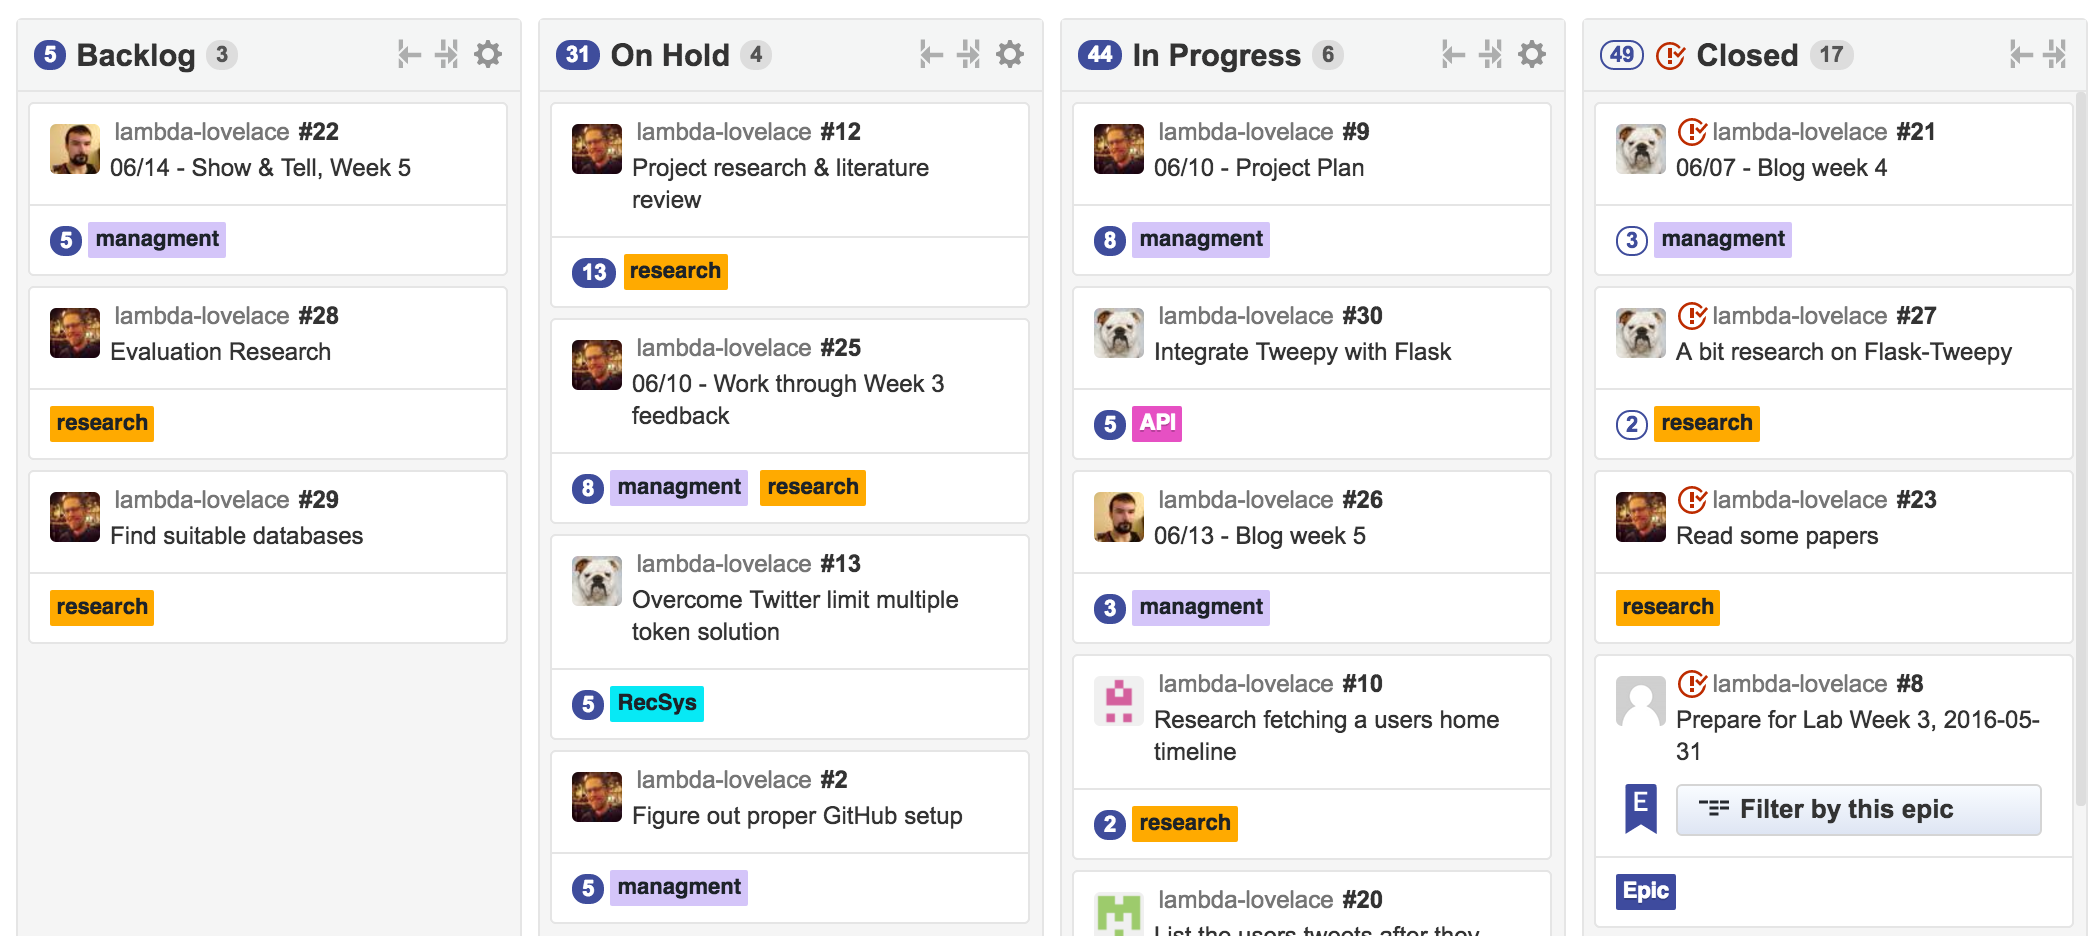
\includegraphics[width=0.8\textwidth]{kanbanboard}  
    \caption{Screenshot from our Kanban board that ZenHub provides}
\end{figure}

\begin{figure}[H]
    \centering
    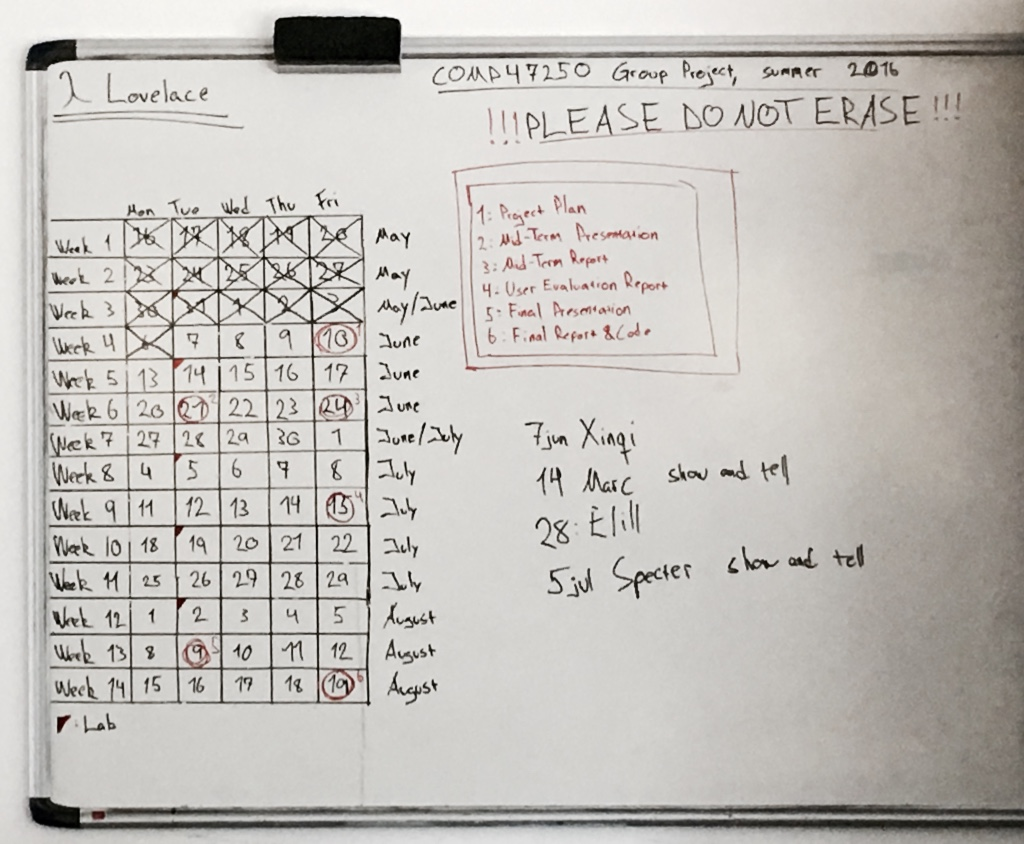
\includegraphics[width=0.8\textwidth]{whiteboard}    
    \caption{A picture of our time schedule whiteboard}
\end{figure}


\newpage


\section{Appenix}
This appendix contains information for a historical perspective such as what Twitter is and who the students and professors are. 

\subsection{Twitter}
Twitter is a microblogging social network where each post or \textit{tweet} is no more than 140 characters in length. A typical Twitter user \textit{follows} multiple other users (followees) and get followed by other users (followers). By following other users they subscribe to all of their tweets and re-tweets (rebroadcast of other user's tweets). The \textit{timeline} is a chronological feed of those tweets.

\subsection{Students \& Professors}
The group project is the third and final semester of the Negotiated Learning MSc in Computer Science at University College Dublin. Here are the students and professors involved:

\begin{samepage}
\begin{center}
\begin{minipage}[t]{.4\textwidth}
	\textbf{Students}:
		\begin{itemize*}
			\item Xinqi Li
			\item Marc Laffan
			\item Junyang Ma
			\item Jón Rúnar Helgason
			\item Eazhilarasi Manivannan
		\end{itemize*}
\end{minipage}
~
\begin{minipage}[t]{.4\textwidth}
	\textbf{Module co-ordinators}:
	\begin{itemize*}
		\item Dr. Georgiana Ifrim
		\item Dr. Brian Mac Namee
		\item Dr. Derek Greene
	\end{itemize*}
\end{minipage}
\end{center}
\end{samepage}

\vspace{0.5em}

\begin{thebibliography}{9} 

\bibitem {vaki}
	$\lambda$ Lovelace blog, \url{http://jonrh.github.io/lambda-lovelace/}
	
\bibitem {ucdgithub}
	Negotiated Learning Project organisation on GitHub \\
	\url{https://github.com/ucd-nlmsc-teamproject}

\bibitem {gitrepo}
	$\lambda$ Lovelace code repository on GitHub \\
	\url{https://github.com/jonrh/lambda-lovelace/}
	
\bibitem {zenhub}
	ZenHub official website \url{https://www.zenhub.com/}


\end{thebibliography}



\end{document}